\section{Input and Output Multiplexer Details}
\label{app:mux_details}

The input demultiplexer and output multiplexer were designed to meet the clock generator's stringent requirements for low jitter, high input-to-output isolation, and minimal area overhead. They route the input clocks to the appropriate frequency path and select the final output for the fine-tuning stage.

\subsection{Input Demultiplexer}
The input demultiplexer was constructed using a two-stage buffer design, where the first stage consists of two identical regular tri-state inverters and the second stage is a common-source inverter stage. PMOS/NMOS common-gate transistors pull the intermediate networks to \texttt{VCC}/\texttt{GND}, respectively. An enable signal controls the tri-state inverters and the intermediate-node pull-up/down networks.

\begin{figure}[htbp]
  \centering
  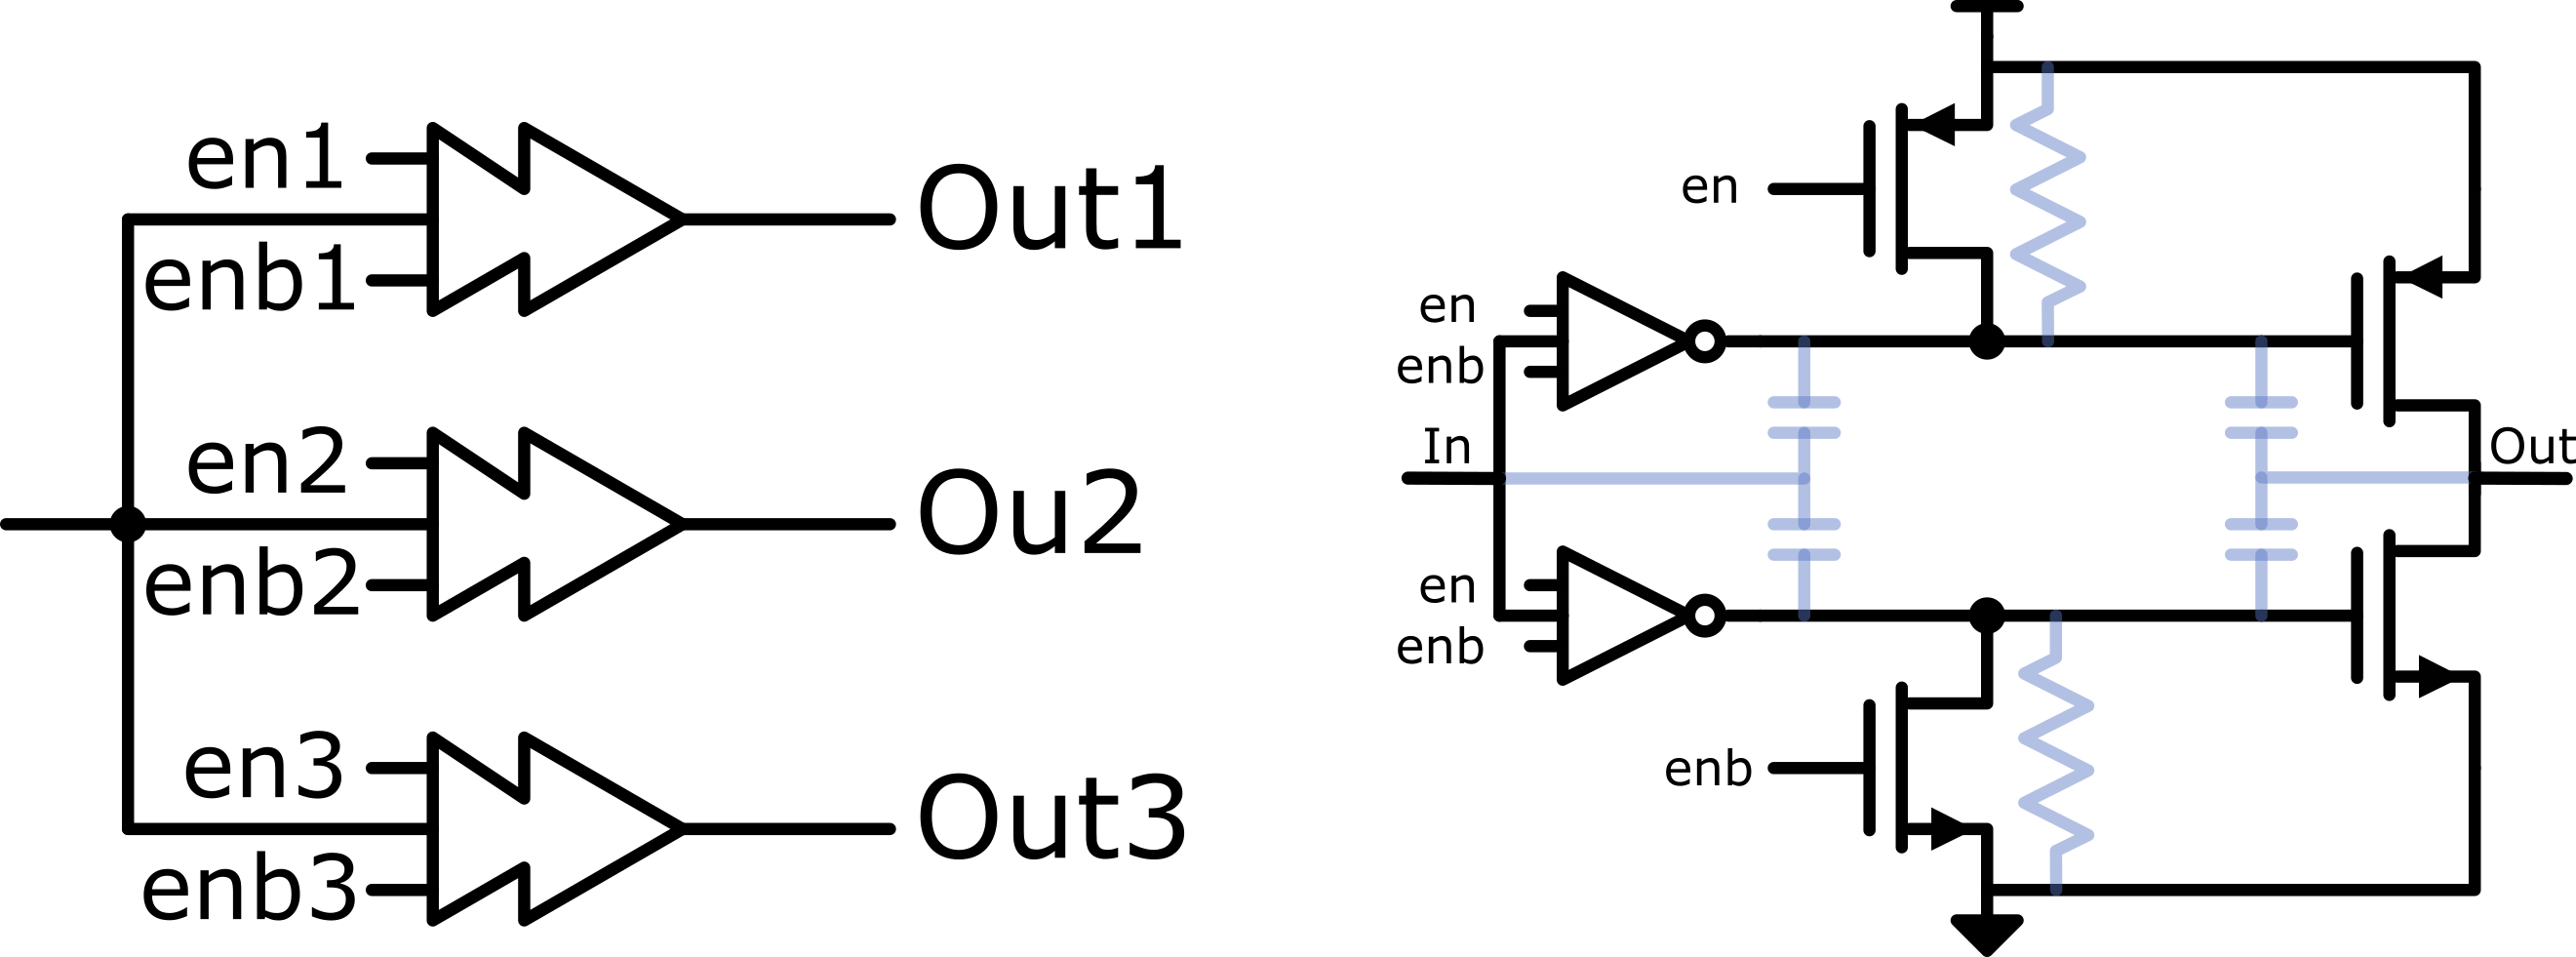
\includegraphics[width=0.8\linewidth]{figures/Schematics/input_demux.png}
  \caption{Input demultiplexer schematic. The first stage consists of two identical tri-state inverters, while the second stage is a common-source inverter stage. PMOS/NMOS common-gate transistors pull the intermediate networks to \texttt{VCC}/\texttt{GND}, respectively.}
  \label{fig:input_demux}
\end{figure}

It is also important to note that since the intermediate nodes are close to the rail voltage, the output transistors are biased in the cutoff region and small voltage changes below \(V_\text{th}\) at the gate will not result in \(I_\text{DS}\) at the output.

\subsection{Output Multiplexer}
The schematic of the output multiplexer is shown in Figure~\ref{fig:output_mux}. The design uses two simple T-Gate switches to select between the high-frequency and mid/low-frequency outputs. A 1-bit control signal and its complement select which switch to close, allowing one of the two inputs to be connected to the output. The T-Gate switches are designed to minimize introduced jitter and ensure adequate isolation between the two output paths. They are sized to have low on-resistance, minimizing voltage drop across the switch and ensuring that the output signal remains close to the rail voltage.

\begin{figure}[htbp]
  \centering
  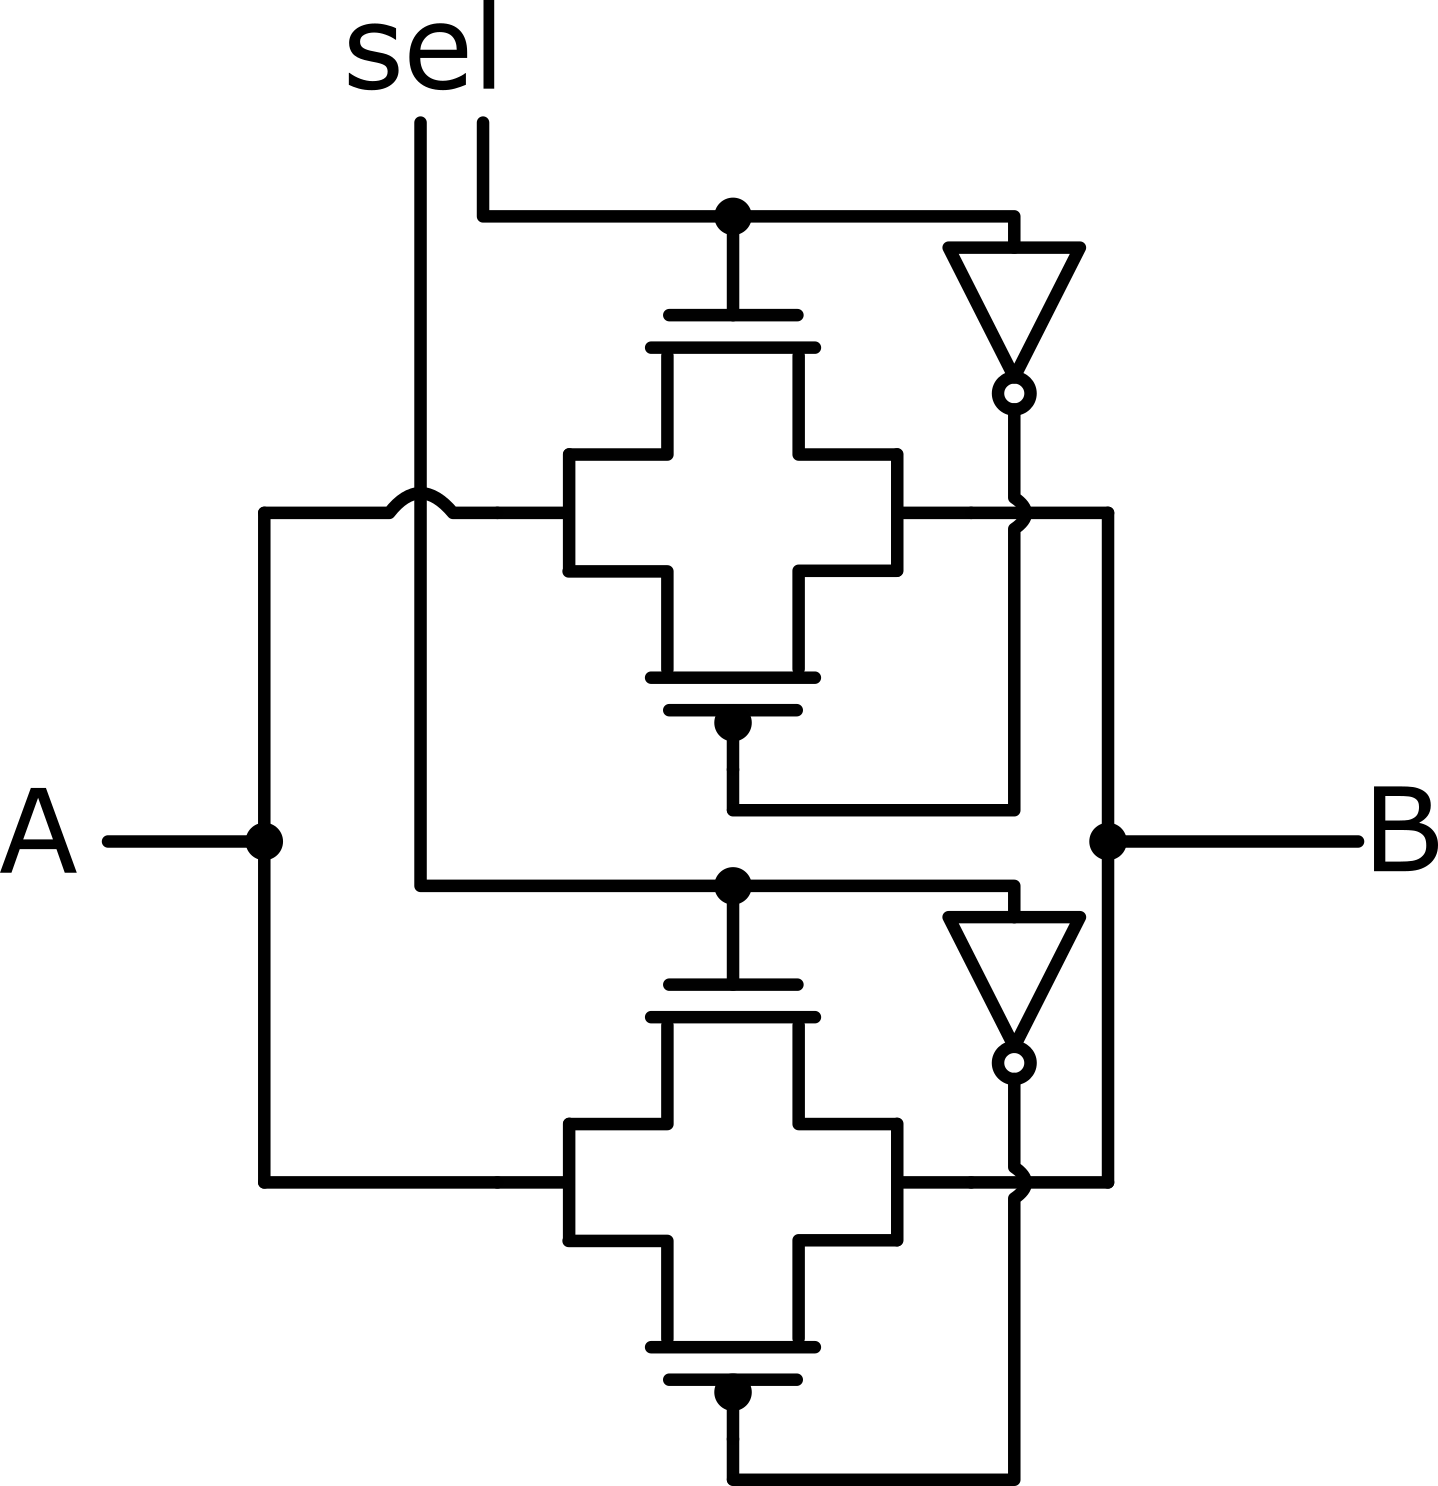
\includegraphics[width=0.3\linewidth]{figures/Schematics/output_mux.png}
  \caption{Output multiplexer schematic. The design uses two T-Gate switches to select between the high-frequency and mid/low-frequency outputs. A control signal selects which switch to close, allowing one of the two inputs to be connected to the output.}
  \label{fig:output_mux}
\end{figure}

